\chapter{Design, Methodology \& Implementation - 25\%}
% This chapter describes the design, methodology and implementation for this project, and the reasoning for the decisions taking throughout this project, connecting the information from the last chapter to this project.

This chapter ties the material from the previous chapter to this project by outlining its design, technique, and execution as well as the rationale behind the choices made along its course.

\section{General Design and Methodology}
Function merging is a powerful compiler optimisation technique that reduces code size by combining similar functions, but its effectiveness depends heavily on identifying which function pairs are suitable candidates for merging. Current heuristic-based approaches often miss opportunities for optimisation or waste compilation time attempting to merge incompatible functions. This project aims to improve function merging in compilers by leveraging machine learning to predict function pairs that are likely to produce beneficial merges.

For this approach to succeed, comprehensive training data needs to be collected consisting of diverse function pairs and their merging performance. These functions will be encoded into a vector representation using IR2Vec to quantify the function's semantic meaning and multiple merging scores which are calculated by F3M's artifacts are contenders for quantify the merging performance. The collected data will require some processing to normalise before being used to develop, train and evaluate different ML models. The training process will involve feeding these vector representations into a neural network architecture that can effectively compare function pairs' encodings and predict their merging compatibility to improve the compiler's function merging decisions.

The project methodology is structured around three interconnected stages: data collection, machine learning model development, and integrating everything together.

The first stage involves collecting data, since effective machine learning benefits from representative data. This involves gathering two essential components: a suitable vector encoding of functions that captures their semantics and a metric that quantifies the similarity between function pairs to determine whether merging would be beneficial. \todo{Talk about the merging outcomes of F3M as well: Successful merges, new merged function size}.

In the second stage, various machine learning architectures are explored and fine-tuned using the collected data to evaluate their performance in predicting merge suitability. This experimentation allows us to identify the most effective model architecture for function merging.

In the final stage, the trained models and function encodings are integrated into the LLVM compiler and evaluated on a suite of benchmarks to measure it's performance in terms of code size reduction of the overall system.

The subsequent sections elaborates on each stage of this process, providing insight into the design decisions and implementation details. Furthermore this project also includes artefacts for reproducing results, including a set-up script to facilitate easy set up which will be detailed at the end of this section.

This project also includes artifacts for reproducing results, including a set up script which will be detailed in the subsequent sections along with elaborations on each stage of this process, providing insight into the design decisions and implementation details.

\todo{Include image of the overall pipeline of the project.}

\section{Data Collection}
To collect the function merging data, the previous SOTA function merging implementation, F3M, was executed on a suite of benchmarks: cc1plus, chrome, libreoffice, linux, llvm, Spec2006, and Spec2007 which were provided in F3M's artefacts as LLVM bitcode (\ref{LLVM:Bitcode}).

\subsection{Use of IR2Vec} \label{subsection:UseOfIR2Vec}
As mentioned in Section \ref{subsection:SemanticalRepresentations}, it is important to encode functions in a way that accurately captures their underlying semantics. To accomplish this, \textbf{\textit{IR2Vec}} was employed to transform the intermediate representation (IR) of each function into a 300-dimensional vector embedding. This wider dimensionality allows the encoder to capture more detail for each function and this process also produces a distinct embedding for every individual function making it a perfect fit for our needs to work at function-level granularity.

IR2Vec was selected for this project because of its proven ability to capture both the semantic meaning and flow of LLVM IR through flow analyses.\cite{IR2Vec}. Its efficient encoding process and graceful handling of out-of-vocabulary tokens via seed embedding vocabulary further contribute to its appeal as an encoder. Moreover, IR2Vec is fully open-source, facilitating straightforward customisation and extension. Furthermore, IR2Vec is available across multiple platforms, it can be utilised as a Python library, a C++ library, or even as a stand-alone binary. This flexibility ensures seamless integration into various development environments, simplifying the overall implementation of the project.

\subsection{Database Solution}
Prior to collecting any data, it was necessary to determine a suitable storage solution which fits the project's needs.

\paragraph{SQL vs CSV} \textbf{\textit{SQL}} databases offer significant advantages over simple file structures like \textit{CSVs} primarily due to the expressive power of the SQL query language. Rather than reinventing the wheel each time a complex query is required, SQL provides a rich set of built-in functions and operators for users. This expressiveness not only simplifies the process of querying but also enhances performance, especially when working with large volumes of data, by leveraging optimised indexing and storage mechanisms. Furthermore, the relational nature of SQL databases, where data is organised into interconnected tables, enables more efficient modifications and queries across related data sets, reducing redundancy and improving maintainability.

\paragraph{SQLite vs PostgreSQL} \textbf{\textit{SQLite}} was selected over other SQL solutions, such as \textit{PostgreSQL} primarily for its ease of use and minimal configuration requirements. Unlike PostgreSQL, which typically requires extensive setup, including robust security configurations and server management, SQLite operates as a server-less, file-based database, making it an ideal choice when sensitive data is not a concern. Additionally, SQLite provides a C++ interface, which is the language used to build LLVM and F3M. Finally, its widespread adoption in the Python ecosystem offers an advantage, popular libraries like \textbf{\textit{Pandas}} and \textbf{\textit{TensorFlow}} provide support to read data from SQLite directly, further simplifying the project's implementation by enabling straightforward connections and interactions.

\subsection{Database Design} \label{subsection:DatabaseSchema}
The design of this database schema is guided by the need to efficiently store and query data, especially since the number of function pairs scales quadratically to the number of functions in a program.

\begin{figure}[tbh!]
\centering
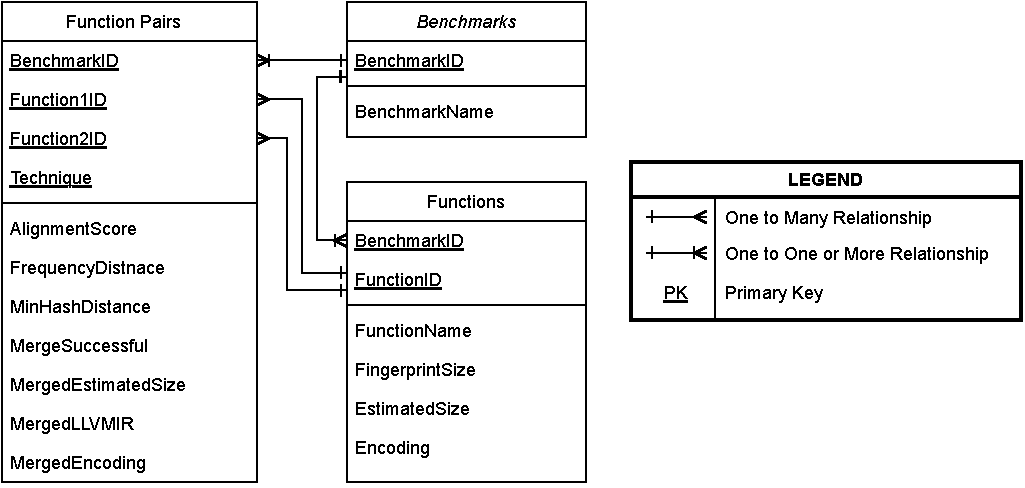
\includegraphics[scale=0.85]{Figures/DataCollectionSchema.pdf}
\caption{Schema of database used to store collected data using crows foot notation}\label{fig:DatabaseSchema}
\end{figure}


The schema consists of three primary tables, as illustrated in Figure \ref{fig:DatabaseSchema}. The \textbf{Benchmarks} table serves as the top-level reference point for all data points. This design ensures that each dataset being evaluated is logically isolated, facilitating independent analyses, comparisons, and debugging if needed.

The \textbf{Functions} table captures detailed information about individual functions for each given benchmark. Combining \textit{BenchmarkID} and \textit{FunctionID} as composite keys ensures that function identifiers are scoped locally within each benchmark, preventing cross-function ID collisions. The foreign keys ensure that each function entry is associated with a valid benchmark. All metadata fields remain optional to support flexible, use‑case‑driven data collection.

For each function, the function's name is recorded as a unique key for linking F3M outputs to IR2Vec embeddings. The fingerprint size is computed as the sum of the frequencies of opcodes in HyFM's function fingerprints, as described in section \ref{HyFM:FingerprintDistance}. Function size is then estimated by summing LLVM’s per‑instruction code‑size costs, queried via the TargetTransformInfo interface.

The functions' encoding are stored as BLOB type to store a pickled Python list representing the function's vector encoding. This decision aims to reduce redundant data transformations since the encodings are generated and used in Python (during training), storing them directly in binary format avoids unnecessary conversions and parsing to and from string representations.

Finally, the \textbf{FunctionPairs} table stores all function pair comparisons. The foreign keys ensure that referenced benchmarks and functions exist. This table only uses a single BenchmarkID alongside two function IDs because function merging is only performed within the same program. This table also stores the distance metrics, AlignmentScore (\ref{METRIC:AlignmentScore}), FrequenceDistance (\ref{HyFM:FingerprintDistance}), MinHashDistance (\ref{METRIC:MinHashDistance}) and merging outcomes. The merging outcomes are optional fields, as if a merging attempt fails, there is no merged function to get information from.

\subsection{Data Collection Framework}
The data collection step was split into two steps, one to collect F3M's merging attempts information and one to collect the functions' embeddings from IR2Vec.

For both steps, two automated scripts were made for each step, where they both share a lot of similarities. A base directory of the benchmarks would be specified by the user, and the script would dive into the directory and sub-directories looking for $\_main\_.\_all\_.\_files\_.\_linked\_.bc$ files, which are bitcode files for the benchmarks. For each bitcode file, the benchmark's name is determined by examining the name of its parent directory. The scripts also has an additional input to specify the database's name and path, ensuring that different runs remain separate if the user wishes to keep them organised. Moreover, the parameters allow multiple shell sessions to run the same script concurrently on different benchmarks, enabling several benchmark data collections to occur simultaneously. This concurrent execution saves time since each script processes benchmarks sequentially. Additionally, this design prevents the corruption of a single SQLite file, as the scripts do not incorporate concurrency controls for simplicity.


\subsubsection{Collecting F3M Merging Metrics}
The collection of merging metrics was intended to be done before collecting function encodings, since not all functions touched on by IR2Vec would be merged in F3M.

To collect merging metrics, SQLite's C++ interface had to be integrated into F3M's implementation within the LLVM codebase. Initially, a SQLite database is initialised with the user-specified name, and F3M's reporting feature is repurposed to pipe the pairwise metrics into the initialised database instead of the terminal.

After obtaining the benchmark name and bitcode file location for each benchmark from the script mentioned above, the script changes its working directory to the bitcode file's directory and executes a \textbf{\textit{make}} command to run each benchmark using F3M's binary, passing the benchmark's name to the compiler via environment variables.

After running the scripts from this step, all fields in the new database should be populated except for the encoding field, which will be populated in the next step.

\subsubsection{Collecting IR2Vec Function Encodings}
The function encodings collection was segregated into a separate step because function encodings only need to be collected once per function, whereas the merging metrics collection processes each function quadratically.

After locating each benchmark's bitcode file using the script mentioned above, IR2Vec's binary was used to generate function-level embeddings from the bitcode files, which were then stored in a text file.

Then the script opens the text file and loads the embeddings into a Python dictionary, with the keys being the function names and the values being the embeddings, parsed into Python lists and serialised into a binary object using the Python Pickle library.

Next, using the database path and the benchmark name, the IR2Vec collection script accesses the database and retrieves the benchmark ID corresponding to the benchmark name, along with all associated function IDs and their function names. These retrieved function names are then matched with the function encodings generated by IR2Vec. Using this matched information, the relevant embeddings are extracted from the dictionary and inserted into the database.

During this process, an issue was identified: the function names used by IR2Vec and LLVM were different. Specifically, LLVM's function retrieval returns mangled names, while IR2Vec produces demangled names. Consequently, IR2Vec's source code was modified and rebuilt to conform to LLVM's naming convention.

\todo{Show an example of before and after of modifying IR2Vec's codebase}

\subsubsection{Merging Data}
Due to the fact that multiple scripts could be run concurrently while writing to different databases, there is a need to merge all data into a single, centralized database. The script accepts a variable number of arguments specifying the input databases to combine and an argument for the new database's name. It works by initialising a new database using the specified name, connecting it to each of the existing databases, and then copying over the information.

\section{Model Development}
To develop machine learning models, the data from the previous step are pre-processed and partitioned to form a representative dataset. Then, two model architectures were designed based on carefully considered rationale. Finally, a framework was established to support efficient training, testing, fine-tuning, and evaluation of these models, streamlining experimentation and providing a reliable structure for iterative improvements.

\subsection{Data Pre-Processing}
\subsubsection{Data Imbalance} \label{Design:DataImbalance}
A major challenge encountered with the dataset was the overwhelming number of function pairs with an alignment score of 0. In total, there were \textbf{\textit{2.2 billion}} function pairs collected, of which \textbf{\textit{1.67 billion}} samples had an alignment score of 0 (zero-samples), \textbf{\textit{1.7 million}} had an alignment score of 1 (one-samples) and \textbf{\textit{570 million}} has an alignment score between 0 and 1 (non-zero-non-one samples). If this imbalance is not properly addressed, the model would likely learn to predict 0 for most situations to achieve a superficially low error, but produces unhelpful predictions.

This imbalance is mitigated in two ways. First, a large portion of the zero samples is discarded so that the number of remaining zero samples equals the combined total of one samples and non-zero-non-one samples. This balancing strategy reduces the dominance of zero samples and decreases overall training time by lowering the total number of training examples. After this step, the following condition holds true:
$$Zero\ Samples = One\ Samples + Non\_Zero\_Non\_One\ Samples$$

Secondly, during model training, each remaining zero-alignment sample is assigned a weight of \textbf{\textit{0.001}}. This weighting means that every non-zero alignment sample contributes 1,000 times as much to the loss function as a zero-alignment sample, thus diminishing the influence of the overly abundant zero samples. In this way, the model is incentivised to learn accurate predictions for non-zero alignment scores.


\subsubsection{Data Split} \label{Design:DataSplit}
After collecting and processing the data, we end up with \textbf{\textit{1.1 billion}} function pairs. The order of data is then randomised to make it diverse when encountered by the machine learning model. After which the dataset is split into three smaller SQLite datasets, the training, validation and testing datasets, each making up 70\%, 10\% and 20\% of the pre-processed dataset respectively. The training dataset is used by the model to train itself, while the validation set is used by the model to tune its hyperparameters (discussed in section \ref{subsubsection:HyperparameterTuning}) and the test set is then used to test the model's performance on unseen data.

Pre-splitting the dataset accelerates training by eliminating the need to determine the data split during runtime. Furthermore, maintaining a permanent split throughout the model development stage reduces uncertainty in performance evaluations, as the deterministic nature of the split ensures consistent results, consequently any changes in metrics could be mainly attributed to the model's performance.

\todo{Add a bar graph of the frequence of the values in the dataset}

\subsection{Hyperparameter Tuning} \label{subsubsection:HyperparameterTuning}
% \subsubsection{Hyperparameter Tuning} \label{subsubsection:HyperparameterTuning}
Due to the sheer volume of training data available, tuning the hyperparameters using the entire training dataset would be computationally prohibitive. Therefore, a subset of 300 million training samples is used for the hyperparameter tuning stage. During this phase, a dedicated validation set is employed to evaluate each configuration of hyperparameters, ensuring that the model’s performance is robust and generalises well, not overfitting to the training data. Once the optimal hyperparameters are identified through this procedure, the model will be retrained on the full dataset comprising 1.1 billion training samples using these optimal settings.

For the hyperparameter optimisation, \textbf{\textit{Optuna}} is employed. Optuna is an efficient, automatic hyperparameter optimisation framework that utilises Bayesian optimization methods to navigate the hyperparameter space. Each evaluation of a particular set of hyperparameters is referred to as a \emph{trial}. During each trial, the model is trained on the subset of data, and its performance is measured on the validation set, specifically its mean squared error. The results from numerous trials guide the search process, balancing exploration of new configurations and exploitation of known good regions in the hyperparameter space, ultimately converging towards a trail with the lowest mean squared error with the optimal settings.

\subsection{ML Model Design}
In general, the machine learning model developed will take in two function's embeddings as inputs and produce an alignment score as the output.

The alignment score provides a robust distance metric for function merging by capturing the structural and semantic correspondence between code sections, discussed in section \ref{METRIC:AlignmentScore}. The alignment-based approaches excel at detecting semantically equivalent code regions despite variations in the implementation. Furthermore, the score gives an early insight into the potential code size reduction achieved through merging the function pair as it measures how well two functions overlap. 

\subsubsection{Dot Product Siamese Model}
This is an implementation of the Siamese network discussed in section \ref{ML:SiameseNetwork}, which uses a shared encoder to process two function encodings and then comparing them using a dot product similarity.

\paragraph{Shared Encoder} The shared encoder is used to produce embeddings for both inputs within the same feature space, transforming the IR2Vec's embeddings into an embedding that facilitates the comparison of the generated embeddings by dot product.

The shared encoder first expands IR2Vec's 300-dimensional vector in 512 dimensions to try and capture any more semantics that was lost due to the limited amount of elements, followed by a dropout layer with a dropout rate of 16.6\% to prevent overfitting. Then a dense layer compresses the new 512 dimensions into 128 dimensions to abstract and keep the most relevant information for the comparison task.  Then batchnormalisation is used to <reasoning> and using this means one less hyperparameter to training compared to using a regular normalisation layer.

The dot product of the two new embeddings are calculate before passing it to a dense layer of 1 unit with a sigmoid layer to map the dot product to a 0 or 1 range to match the alignment score's range.

The shared encoder is used to produce embeddings for both inputs within the same feature space, transforming the IR2Vec's embeddings into a more comparable representation that enhances the comparison of function pairs by dot product.

The shared encoder first expands IR2Vec's 300-dimensional vector to 512 dimensions to capture richer semantic information that might be constrained in the original representation, followed by a dropout layer with a dropout rate of 16\% to prevent overfitting. Then a dense layer compresses the expanded 512 dimensions into 128 dimensions to abstract and keep the most relevant information for the comparison task. 

After this, batch normalisation is applied to standardise the layer outputs, which helps stabilise and accelerate the training process by reducing internal covariate shift. Using batch normalisation also reduces the need for careful initialisation and allows higher learning rates, effectively requiring one less hyperparameter to tune compared to using a regular normalisation layer.

\paragraph{Score Generation}
Once both function embeddings have been processed through the shared encoder, their dot product is calculated to measure the similarity between them, capturing how aligned the two functions are in the embedding space. This similarity value is then passed through a dense layer of 1 unit with a sigmoid activation function to map the dot product to the [0,1] range, corresponding to the desired alignment score range.

\subsubsection{Multi-headed Self-Attention Model}
This is an implementation of a model which tries to take advantage of the attention mechanism discussed in section \ref{ML:AttentionMechanism}.

The model first processes each IR2Vec 300-dimensional embedding through a shared dense layer with 512 units and ReLU activation, expanding the representation to capture richer semantic information. Unlike the Siamese model, these expanded representations are then reshaped and concatenated to form a sequence of two tokens, allowing the model to treat the function pair as a unified sequence.

The core of this architecture is the transformer encoder block, which implements multi-head self-attention with 4 attention heads, each with a dimension of 64. This mechanism allows each function representation to attend to the other, capturing complex relationships between their features. 

The self-attention output passes through dropout (30\%) to prevent overfitting and uses skip connections and layer normalisation to stabilise training. The subsequent feed-forward network with ReLU activation further processes these attention-weighted representations through a dimension of 64 before returning to the original dimension. After the transformer encoding, the model applies global average pooling to aggregate the sequence information into a single vector representation. This condensed representation is then passed through a final dense layer with sigmoid activation to produce an alignment score in the [0,1] range, where higher values indicate better candidates for function merging.

By leveraging attention mechanisms instead of simple dot products, this model can potentially capture more nuanced relationships between function pairs, learning which aspects of functions are most relevant for aligning functions.


\subsection{Framework/Pipeline for Model Development}
This section discusses the framework design and explains key design decisions.

\subsubsection{Serialising Data}
Initially, the models loaded data using Tensorflow's dataset interface which acts as a lazy iterator, querying the SQLite dataset. Tensorflow's SQL dataset interface could not be used, because the encodings which were stored as BLOB objects required depickling before being loaded into the model.

Direct querying of the SQLite dataset proved extremely slow. Therefore, with assistance from my supervisor, Pavlos, a script to serialise the data into \textbf{\textit{NumPy}} arrays was created. This approach significantly reduced the number of processing operations required, resulting in faster loading and processing times compared to SQL querying.

The serialisation utilises two two-dimensinal \textit{NumPy} arrays: one to store function encodings and another to store alignment scores. For the encodings array, each unique tuple (BenchmarkID, FunctionID) is assigned a new unique function ID. These function IDs are stored with their respective encodings occupying the remaining columns.

The second array stores alignment scores of function pairs using three columns: the first function's unique ID, the second function's unique ID, and the pair's alignment score. Without formal measurements, this method was observed to decrease training time by approximately 60\% in small test cases.

The \textit{NumPy} arrays are saved to binary files for direct loading when needed. While the number of functions is manageable, it pales in comparison to the number of function pairs. Therefore, the array storing pairwise metrics must be split into multiple binary files of specified number of points while the array storing function encodings can be contained in a single file.

Selecting an appropriate chunk size during serialisation is crucial, as excessively large values can cause system crashes. The script verifies that at least 20\% of system memory is available before retrieving the next data batch. If insufficient memory is available, the script sleeps until adequate memory becomes available. A potential deadlock can occur if the script holds data in memory while waiting to meet chunk size requirements but lacks sufficient memory to retrieve the additional data needed.

\todo{ADD A PICTURE OF THE SERIALISED DATA}

\subsubsection{Loading Data}
This process utilises the TensorFlow dataset interface, where the dataloader first loads all function encodings into memory by storing them into a \textit{Python} dictionary, then processes each chunk of pairwise metrics by replacing unique function IDs with their corresponding encodings.

This loading process was observed to be time-intensive. To address this performance bottleneck, the \textbf{\textit{concurrent}} Python library was implemented to load the next data chunk in a separate thread while the model trains on the current available data. These loaded chunks are placed in a queue which the dataloader lazily iterates through, significantly reducing the time the model spends waiting for data preparation between chunks and thereby accelerating the training process.

The data loader is configured to process only one additional file concurrently, as processing more files simultaneously provides no performance benefit and consumes excessive system memory. This is particularly important since each fully expanded input contains 601 32-bit float values, around 2KB (\ref{Calculation:InputSize}).

To prevent system crashes due to memory exhaustion, the loader verifies that at least 20\% of system memory is available before loading and expanding each new data chunk. This memory management strategy ensures stable operation throughout the training cycle.

\subsubsection{Running the Model}
To steamline the process of model development, a centralised script was developed that efficiently handles both training and hyperparameter tuning across different model architectures. The main script accepts various command-line arguments to specify the model type, the operational mode (training or hyperparameter tuning), the location to saved the trained models to and when in training mode, the specific model parameters.

For this modular approach to function effectively, each new model must implement two standard interface functions: $get\_model()$ and $HyperParameterTraining()$. The $get\_model()$ function provides the main script access to the model, while $HyperParameterTraining()$ encapsulates any model-specific hyperparameter optimisation requirements. This standardized interface eliminates redundant code and significantly simplifies working with different model designs.

For model evaluation and result visualisation, a \textbf{\textit{Jupyter Notebook}} was created. This notebook tests trained models against the test dataset, calculates the mean squared error, and generates comparative plots of predicted versus true alignment scores to visually demonstrate model performance.

\section{System Integration}
This section describes how IR2Vec and the trained ML models were integrated into the F3M's codebase to leverage the ML model's heuristics for function merging decisions.

\subsection{Integrating Tensorflow}
The initial integration strategy involved using \textbf{\textit{PyBind}} to load the trained TensorFlow models into the compiler. This approach was selected because one variant of the Siamese Model had been developed using the L1 distance metric instead of the dot product. Since this implementation required a custom layer not natively available in TensorFlow, PyBind appeared advantageous for running python code, therefore allowing the use of custom layers.

However, PyBind consistently crashed when attempting to load TensorFlow models. Given these limitations, \textit{TensorFlow's C++ API} was adopted as an alternative solution for loading the trained models. This decision required abandoning the L1 distance Siamese model due to the engineering work required to support its custom layer in the new integration approach.

\subsection{Integrating IR2Vec} \label{Design:IntegratingLLVM}
Next, since IR2Vec was developed in C++, the initial approach involved incorporating its header files and source code from the official \textit{GitHub} repository. However, while testing the project, errors occurred whenever the compiler attempted to request embeddings from IR2Vec. This compatibility issue likely stemmed from version differences between the LLVM versions used by each project. IR2Vec was based on LLVM 18.1.8 at the time of this project, while F3M used version 18.0.0, necessitating an alternative solution.

The adopted workaround involved pre-generating function encodings using IR2Vec's stand-alone executable for the benchmarks and storing them in text files. During compilation, the system would then only need to parse these files and load the encodings into a map for quick encoding lookup of each function.

This integration approach imposed a significant limitation: newly generated merged functions could not be considered as candidates for further merging, as it was not possible to obtain embeddings for these new functions during compile time. This constraint restricted the optimisation potential to a single pass of function merging.

\subsection{How it all fits together}
The function merging process begins when all candidates are placed into a priority queue. As each candidate is processed, it is removed from the queue for assessment. The queue prioritises functions with larger fingerprint sizes, giving them precedence over smaller ones. During assessment, the system predicts the alignment score between the current function and all other candidates in the queue. Merging is then only attempted with the function that yields the highest predicted alignment score.

\paragraph{Thresholding Alignment Score} Not all highest predicted score functions are merged, only if the alignment score is higher than a pre-determined threshold value. This was added because a function could be unsuitable to merge with all other functions, and we would like to skip it instead of wasting compiling time on unprofitable merges. Multiple thresholding values were tried, 0.4, 0.5, 0.6.

\paragraph{Thresholding Alignment Score} Even when a highest-scoring function pair is identified, merging only proceeds if the alignment score exceeds a pre-determined threshold value. This threshold mechanism prevents wasting compilation resources on unprofitable merges when a function may be unsuitable for merging with any other functions in the queue. During system evaluation, multiple thresholding values were tested, including 0.4, 0.5, and 0.6, to determine the optimal balance between merge opportunities and compilation efficiency.

% \section{Artifactory and Set up Script}
% \subsection{Talk about the set up script provided}
% Discuss the artifact being available and the simple set up script. Explain why IR2Vec has to be built individually by the user.

\section{Artifactory and Set up Script}
\subsection{Repository and Accessibility}
All code developed for this project is publicly available as artifacts in a GitHub repository, linked in appendix \ref{Artifacts}. This repository contains the complete codebase, including models, data processing scripts, integration components, and evaluation tools. The repository is structured to facilitate easy navigation and understanding of the project's components, with clear documentation for each module.

\subsection{Automated Setup Script}
To enhance accessibility and reproducibility, a comprehensive setup script has been developed that automates the installation and configuration process. The script applies custom configurations to ensure compatibility between components and prepares the system for immediate experimentation. This automation significantly reduces the technical barriers to reproducing the research, allowing users to quickly begin exploring the function merging improvements.

A detailed README file is included in the repository root, providing comprehensive guidance through the project setup process. The documentation clearly outlines the required dependencies, and tested environments to ensure compatibility. It includes straightforward installation instructions that walk users through the cloning process and execution of the setup script.

The setup script intentionally excludes the complete installation of IR2Vec, instead only cloning the repository and applying necessary patches. This decision was made because IR2Vec requires a local build of LLVM as a prerequisite, which would require extensive disk space and compilation time.













